\section{Conclusions and Future Work}
\begin{figure*}
  \centering
  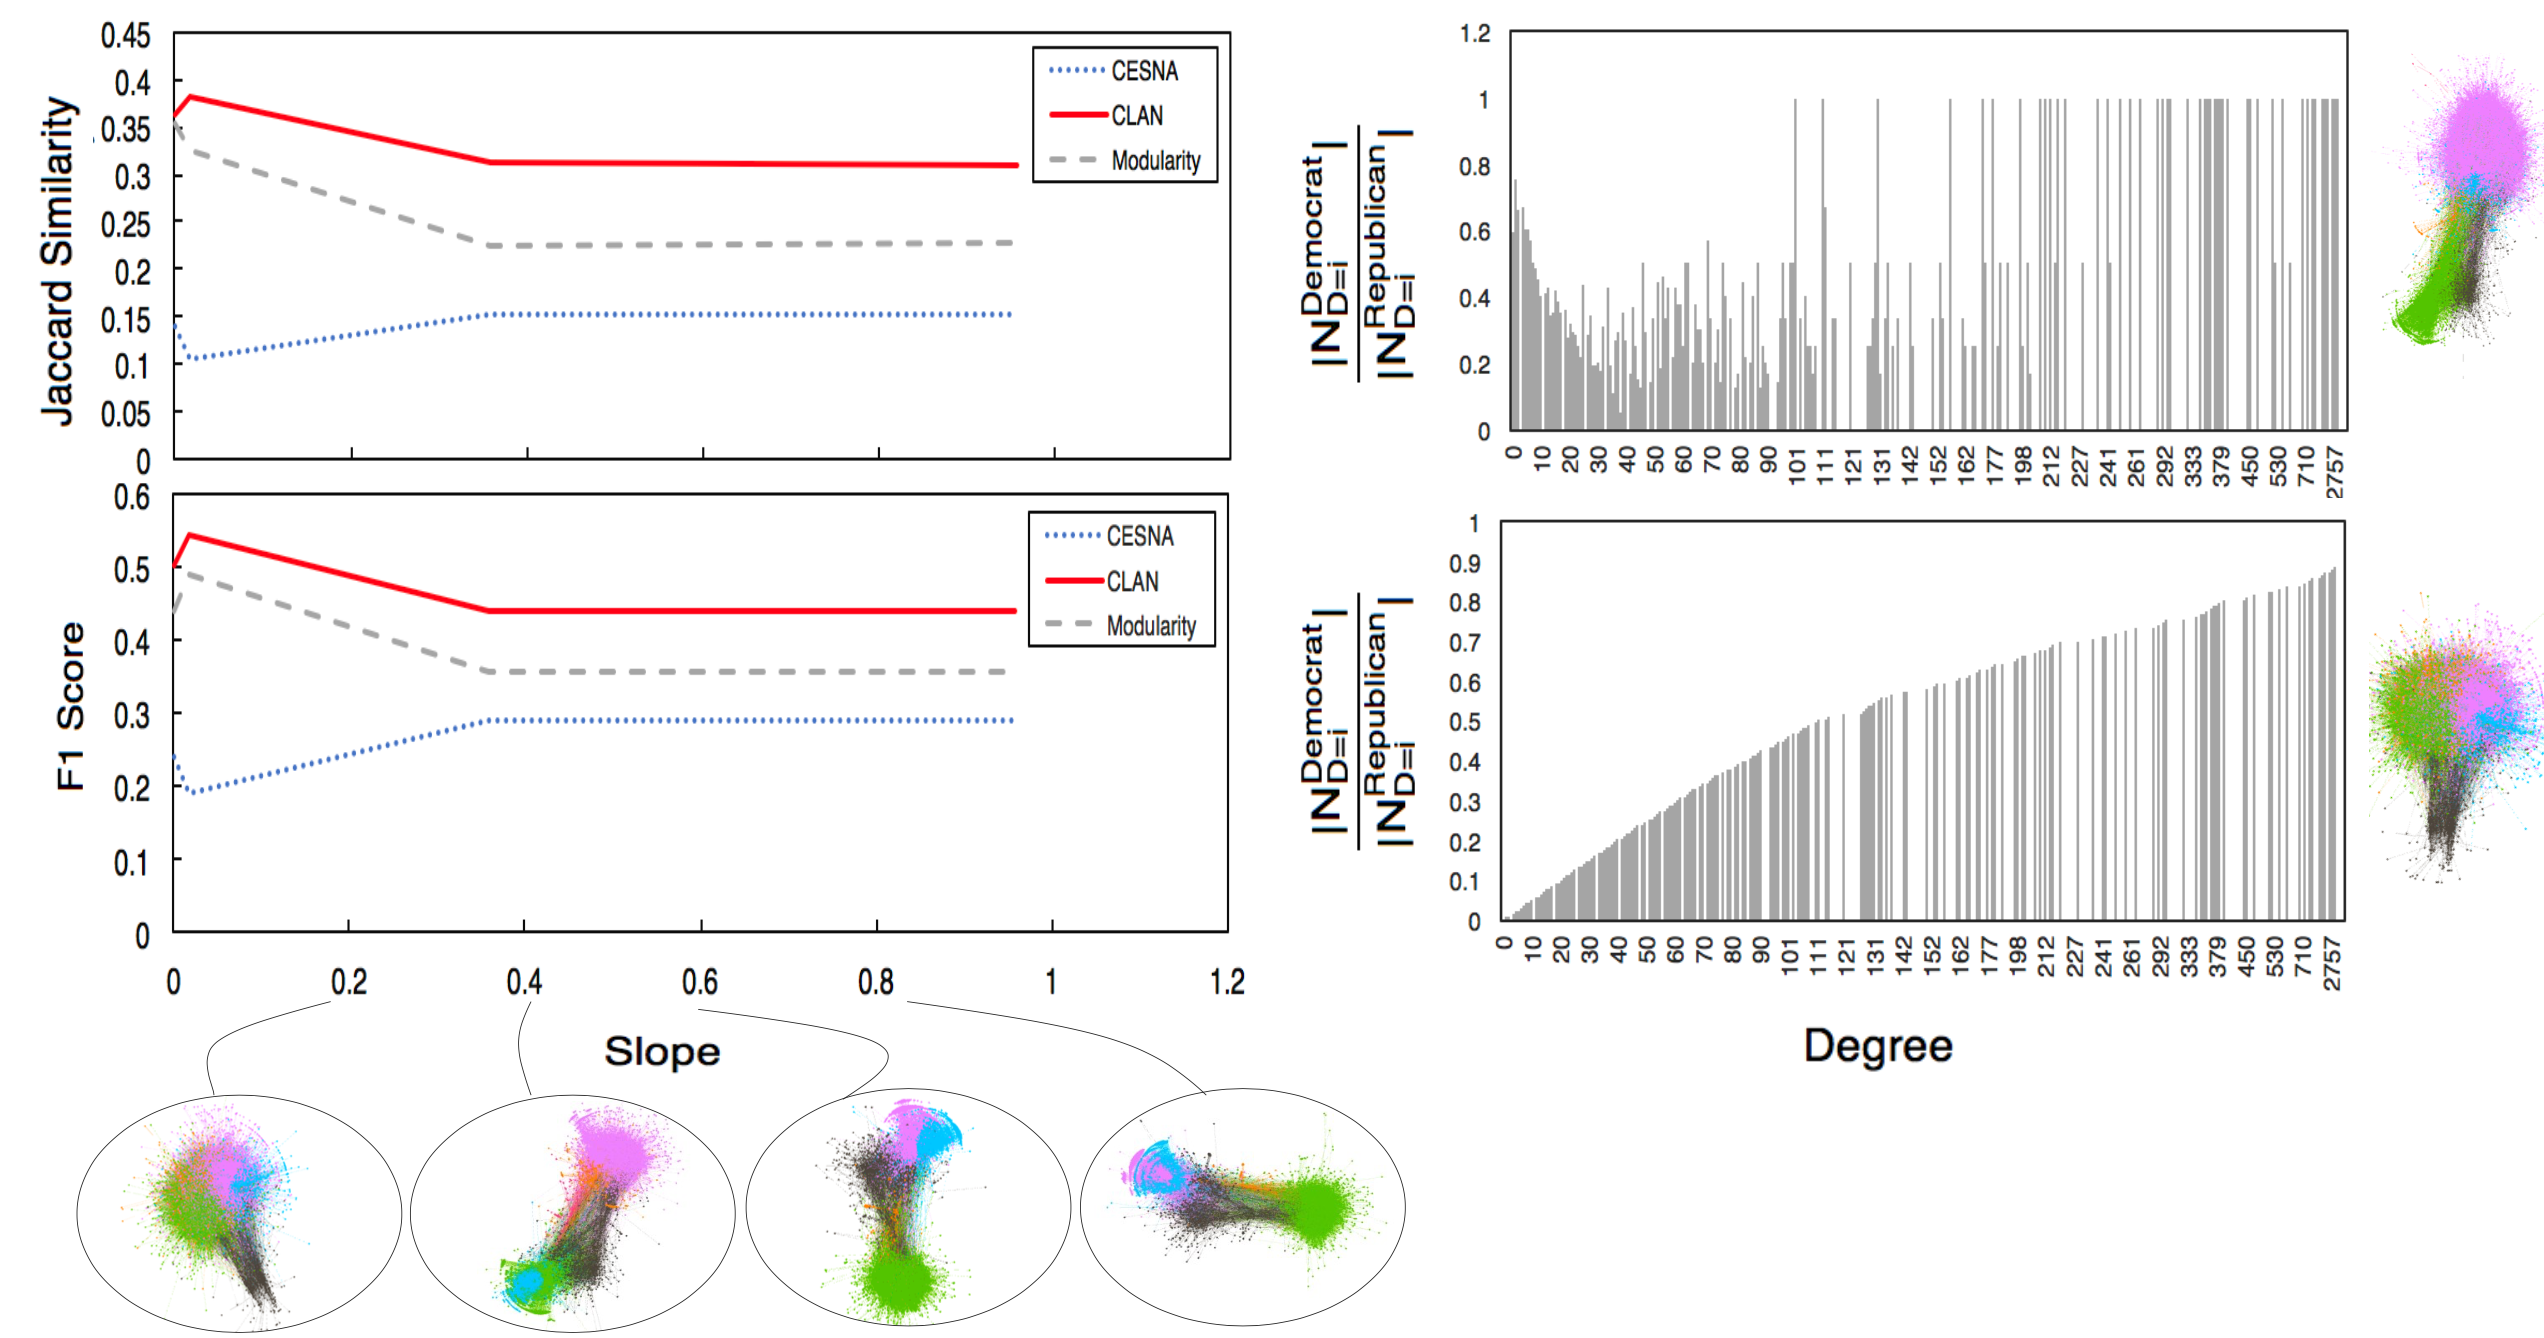
\includegraphics[width=\textwidth]{nex2.png}
  \caption{Synthetic distributions with their corresponding network and obtained results for the 2016 U.S. Presidential Election dataset.}
  \label{synthetic2}
\end{figure*}
In this paper, we introduce a new community detection method that mitigates the bias in existing detection methods that fail to properly account for sparsely-connected nodes in social networks. CLAN minimizes such biases by including the lowly-connected nodes into their true communities. Our empirical results demonstrate that inclusion of those users  enables CLAN to achieve overall superior performance in terms of F1-score and Jaccard similarity. We reported these results by providing evidence through our qualitative and quantitative experiments. Through qualitative analysis, we are able to show that these lowly-connected users, in aggregate, offer information that can be of use for analysis of social network data.

% Additionally, experiments were conducted in this paper both in terms of the ground truth label collection through human annotation and in terms of experiments done to prove CLAN's capability in outperforming the state of the art {\bf repetetive?}. We not only conducted experiments with the labels provided by the human annotators in our Gamergate dataset but also through automated methods in another dataset, the 2016 U.S. Presidential Election dataset, discussed in this paper. The results were then compared against these labels that were collected both through manual labor and automated approaches.

Finally, we show that our method is capable of outperforming other methods not only in real datasets but also in different types of synthetic environments with different population distributions, namely distributions where the users community is correlated with their connectivity. The results reported the performance of methods with regards to F1 and Jaccard similarity scores. 

We see two promising directions for future work. First, to extend this method to introduce a new hierarchical community detection method capable of detecting subgroups within larger communities. Second, we would like to consider edge attributes simultaneously with node attributes to enable this method to consider different types of connections.

\section{Acknowledgments}
This material is based upon work supported by the Defense Advanced Research Projects Agency (DARPA) under Agreement No. HR0011890019. We thank Greg Ver Steeg and Palash Goyal for helpful insights and discussions.
